
\documentclass[11pt,a4paper]{article}
\usepackage[utf8]{inputenc}
\usepackage[T1]{fontenc}
\usepackage[spanish]{babel}
\usepackage[margin=2.5cm]{geometry}
\usepackage{graphicx,tabularx,longtable,array,fancyhdr}
\usepackage[table]{xcolor}
\setlength{\headheight}{14pt}
\setlength{\parindent}{0pt}
\setlength{\parskip}{6pt}
\setlength{\emergencystretch}{1.5em}
\renewcommand{\arraystretch}{1.23}
\pagestyle{fancy}
\fancyhf{}
\fancyhead[L]{\small UTEQ · Ingeniería de Requerimientos}
\fancyhead[R]{\small TA-IND-01}
\fancyfoot[L]{\small Angelo Espinoza}
\fancyfoot[R]{\small Página \thepage}
\usepackage[hidelinks]{hyperref}
\usepackage[backend=biber,style=ieee]{biblatex}
\addbibresource{referencias.bib}

\begin{document}
\begin{center}
    {\large\textbf{UNIVERSIDAD TÉCNICA ESTATAL DE QUEVEDO}}

    Facultad de Ciencias de la Computación\\
    Carrera de Software

    \vspace{0.6cm}
    {\LARGE\textbf{IEEE 29148 y tipos de requisitos}}\\[4pt]
    {\large Análisis de YouTube Web}

    \vspace{0.2cm}
    {\large TA-IND-01}\\
    Actividad sumativa individual
\end{center}

\vspace{0.4cm}
\section{Datos informativos}
\begin{tabularx}{\textwidth}{|l|X|}
\hline
\rowcolor{gray!15}
\textbf{Campo} & \textbf{Detalle} \\ \hline
Estudiante & Angelo Maximiliano Espinoza Pivaque \\ \hline
Asignatura & Ingeniería de Requerimientos (ISR-401) \\ \hline
Nivel y paralelo & Cuarto nivel, paralelo A \\ \hline
Docente & Gleiston Cicerón Guerrero Ulloa, PhD \\ \hline
Caso & YouTube Web \\ \hline
Fecha de entrega & 11 de noviembre de 2026 \\ \hline
\end{tabularx}

\section{Descripción y alcance}
YouTube Web permite buscar, ver y organizar videos desde el navegador.
El análisis se centra en el espectador que usa la plataforma en una
computadora. Se estudian tres recorridos: buscar un tema, reproducir
un video de los resultados y consultar las listas de reproducción.
Como ejemplo se utiliza la búsqueda de contenido sobre jerarquía de memoria.
El ejercicio sigue el encuadre de la asignatura \cite{uteqencuadre}.

\section{Resumen analítico de la norma}
Un requisito transforma una necesidad en una condición que se puede discutir
y comprobar. La cláusula 5.2.4 de ISO/IEC/IEEE 29148:2018 orienta la
redacción del enunciado \cite[cl. 5.2.4]{ieee29148}. Para el caso de
YouTube Web, una forma práctica de aplicarla es identificar el sujeto, el
comportamiento esperado y las condiciones pertinentes. Por ejemplo, la
necesidad de encontrar material para estudiar se puede expresar así:
«Cuando el espectador envíe una consulta de texto, YouTube Web deberá
mostrar la página de resultados de esa consulta». La condición distingue
la búsqueda ejecutada del simple hecho de escribir en la barra.

\subsection{Características de un requisito individual}
La cláusula 5.2.5 propone nueve características para revisar cada
enunciado \cite[cl. 5.2.5]{ieee29148}. Aplicadas al caso, permiten
examinar lo siguiente:

\begin{enumerate}
\item \textbf{Necesario.} Debe responder a una necesidad del espectador.
Pausar un tutorial le permite detenerse para tomar apuntes.
\item \textbf{Apropiado.} El detalle debe corresponder al nivel del análisis.
Para pedir que aparezcan resultados basta describir lo observable en el navegador.
\item \textbf{No ambiguo.} Debe admitir una interpretación clara.
«Tiempo transcurrido» se refiere al punto actual de reproducción.
\item \textbf{Completo.} Debe incluir la información necesaria para entender
qué se espera. Si el requisito trata de una lista personal, conviene indicar
que la sesión está iniciada.
\item \textbf{Singular.} Debe expresar una obligación principal. Pausar
un video y guardarlo en una lista se comprueban por separado.
\item \textbf{Factible.} Debe poder realizarse dentro de las condiciones y
recursos disponibles. Un tiempo de respuesta se plantea para un equipo y
una red concretos.
\item \textbf{Verificable.} Debe permitir reunir evidencia de cumplimiento.
Para comprobar la pausa se observa si el contador deja de avanzar.
\item \textbf{Correcto.} Debe reflejar la necesidad real. Si el espectador
quiere volver a un video, el criterio debe comprobar que puede encontrarlo
en la lista elegida.
\item \textbf{Conforme.} Debe seguir el formato acordado. En esta tarea,
cada requisito tiene identificador, tipo y criterio de aceptación.
\end{enumerate}

Estas características se complementan. Una frase puede ser clara y aun
así estar incompleta si omite una condición decisiva. «Mostrar mis listas»
es comprensible, pero todavía necesita indicar a qué cuenta pertenecen
las listas que se espera ver. Revisar esa condición antes de redactar la
prueba evita que dos personas evalúen situaciones diferentes.

\subsection{Características del conjunto de requisitos}
La cláusula 5.2.6 permite revisar la especificación como un todo
\cite[cl. 5.2.6]{ieee29148}. Para que el conjunto sea \textbf{completo},
debe cubrir el alcance acordado: búsqueda, reproducción y listas. La
\textbf{consistencia} exige que los enunciados usen los términos de forma
estable y que sus condiciones sean compatibles. Por ejemplo, un requisito
puede permitir buscar sin iniciar sesión y otro exigir una sesión para
guardar en una lista personal. Precisar la condición de cada uno permite
interpretarlos en conjunto.

La \textbf{factibilidad} se evalúa también para todos los requisitos
juntos: las metas de rendimiento y facilidad de uso deben poder
comprobarse con un entorno y un método definidos. El conjunto debe ser
\textbf{comprensible}, de modo que el lector entienda qué cubre y cómo se
relacionan sus partes. Por último, debe \textbf{poder validarse} frente a
la necesidad original. Un recorrido de prueba en el que el espectador
busca un tutorial, abre el resultado y lo guarda en una lista permite
revisar si los requisitos, vistos en conjunto, respaldan su objetivo.

\subsection{Lenguaje que conviene evitar}
La cláusula 5.2.7 advierte sobre expresiones que hacen difícil interpretar
o comprobar un requisito \cite[cl. 5.2.7]{ieee29148}. En este ejercicio,
«rápido» o «fácil» requieren una medida. «El mejor reproductor» introduce
un superlativo sin criterio. «Mejor que antes» deja sin identificar la
referencia de comparación, mientras que «si es posible» permite omitir
el comportamiento sin especificar en qué condiciones. Los pronombres
como «esto» pueden perder su referente y expresiones abiertas como
«entre otros» dejan indefinido qué elementos se evaluarán. También
conviene revisar absolutos como «siempre», conectores como «y/o» y
referencias incompletas cuya versión o alcance no se pueda identificar.

Una corrección concreta es reemplazar «la búsqueda debe ser rápida»
por un tiempo máximo para una consulta y un entorno definidos. El tiempo
se mide desde el envío de la consulta hasta que aparece el primer
resultado. El valor elegido es un objetivo del ejercicio, y la prueba
debe registrar el resultado real. Esta distinción permite comparar lo
que el requisito pide con lo que se observa en la plataforma.

\section{Glosario}
Los términos se resumen a partir de la cláusula 3
\cite[cl. 3]{ieee29148}. Los ejemplos corresponden al caso de YouTube Web.

\begin{longtable}{@{}p{.26\linewidth}p{.70\linewidth}@{}}
\rowcolor{gray!15}\textbf{Término y cláusula} & \textbf{Definición y ejemplo} \\
\endhead
Requisito derivado (3.1.10) & Requisito que surge al analizar o precisar otro requisito. Ejemplo: mostrar una lista guardada se deriva de la necesidad de retomar videos después. \\
Desarrollador (3.1.11) & Persona u organización que realiza actividades de desarrollo. Ejemplo: el equipo que implementa los controles del reproductor. \\
Escenario operacional (3.1.17) & Descripción de una secuencia de interacciones en un contexto de uso. Ejemplo: buscar un tutorial, abrirlo y pausarlo para tomar apuntes. \\
Operador (3.1.18) & Persona u organización que opera el sistema. Ejemplo: el espectador que maneja los controles de reproducción en el navegador. \\
Requisito (3.1.19) & Enunciado que expresa una necesidad y las condiciones o restricciones asociadas. Ejemplo: mostrar los resultados cuando se envía una consulta. \\
Obtención de requisitos (3.1.20) & Actividad para descubrir y obtener requisitos de las fuentes pertinentes. Ejemplo: preguntar a estudiantes cómo vuelven a encontrar los tutoriales que guardaron. \\
Trazabilidad de requisitos (3.1.23) & Registro de cómo se deriva un requisito de otro de nivel superior y cómo se asigna a elementos de nivel inferior. Ejemplo: vincular RF-03 con la necesidad de tomar apuntes y con la prueba de pausa. \\
Matriz de trazabilidad (3.1.24) & Tabla que registra relaciones entre elementos. Ejemplo: una fila enlaza RC-01 con la necesidad de buscar contenido y con su prueba de tiempo. \\
Validación de requisitos (3.1.25) & Confirmación de que los requisitos describen el sistema que las partes interesadas necesitan. Ejemplo: revisar con un estudiante si lo especificado le permitiría retomar un tutorial guardado. \\
Verificación de requisitos (3.1.26) & Revisión de que los requisitos están bien formados individualmente y como conjunto. Ejemplo: comprobar que RF-03 define cuándo se pausa el video y permite redactar una prueba. \\
\end{longtable}

\section{Requisitos y criterios de aceptación}
Se distinguen cinco tipos: funcional, interfaz, restricción de diseño,
desempeño y usabilidad. Los dos últimos agrupan los cinco
requisitos de calidad, clasificados según ISO/IEC 25010:2023
\cite{iso25010}. Los umbrales y restricciones son propuestas del ejercicio.
Para las pruebas de tiempo se propone Chrome de escritorio, ventana de
1366 por 768 píxeles y conexión estable de al menos 20 Mb/s de descarga.
En las pruebas del reproductor se usa un video público disponible, una vez
que se pueda reproducir el contenido.

\begingroup
\small
\setlength{\tabcolsep}{4pt}
\renewcommand{\arraystretch}{1.25}
\begin{longtable}{|p{.085\textwidth}|p{\dimexpr.915\textwidth-4\tabcolsep-3\arrayrulewidth\relax}|}
\hline\rowcolor{gray!15}\textbf{Código} & \textbf{Clasificación y criterio de aceptación} \\ \hline
\endfirsthead
\hline\rowcolor{gray!15}\textbf{Código} & \textbf{Clasificación y criterio de aceptación} \\ \hline
\endhead
\textbf{RF-01} & \textbf{Enunciado:} YouTube Web deberá mostrar una página de resultados al enviar una consulta de texto.\newline
\textbf{Tipo:} Funcional.\newline
\textbf{Criterio de aceptación:} Buscar «jerarquía de memoria» y verificar que aparece una página con resultados de esa consulta. \\ \hline
\textbf{RF-02} & \textbf{Enunciado:} YouTube Web deberá abrir el reproductor del video seleccionado desde los resultados.\newline
\textbf{Tipo:} Funcional.\newline
\textbf{Criterio de aceptación:} Elegir un resultado y comprobar que el título abierto coincide con el seleccionado. \\ \hline
\textbf{RF-03} & \textbf{Enunciado:} YouTube Web deberá pausar el video cuando el espectador pulse el control de pausa durante la reproducción.\newline
\textbf{Tipo:} Funcional.\newline
\textbf{Criterio de aceptación:} Pulsar pausa durante la reproducción y comprobar que el contador permanece en el mismo valor durante tres segundos. \\ \hline
\textbf{RF-04} & \textbf{Enunciado:} YouTube Web deberá mostrar las listas de reproducción disponibles para la cuenta con sesión iniciada.\newline
\textbf{Tipo:} Funcional.\newline
\textbf{Criterio de aceptación:} Abrir Playlists con una cuenta que tenga dos listas propias de prueba y verificar que aparecen ambas. \\ \hline
\textbf{RI-01} & \textbf{Enunciado:} YouTube Web deberá mostrar el tiempo transcurrido y la duración total en los controles de un video pregrabado.\newline
\textbf{Tipo:} Interfaz.\newline
\textbf{Criterio de aceptación:} Hacer visibles los controles y comprobar que se muestran ambos tiempos. \\ \hline
\textbf{RI-02} & \textbf{Enunciado:} YouTube Web deberá mostrar el nombre y el conteo de videos en cada tarjeta de lista personal.\newline
\textbf{Tipo:} Interfaz.\newline
\textbf{Criterio de aceptación:} Abrir Playlists y cotejar el nombre y el conteo de cada una de dos listas de prueba con sus respectivas vistas de detalle. \\ \hline
\textbf{RF-05} & \textbf{Enunciado:} YouTube Web deberá reanudar un video pausado al activar el control de reproducción.\newline
\textbf{Tipo:} Funcional.\newline
\textbf{Criterio de aceptación:} Pausar un video, activar reproducción y comprobar que el contador vuelve a avanzar. \\ \hline
\textbf{RF-06} & \textbf{Enunciado:} YouTube Web deberá abrir la vista de una lista al seleccionar su tarjeta.\newline
\textbf{Tipo:} Funcional.\newline
\textbf{Criterio de aceptación:} Seleccionar una lista que contenga un video y comprobar que se muestra ese video en la vista abierta. \\ \hline
\textbf{RD-01} & \textbf{Enunciado:} El recorrido de búsqueda y reproducción deberá poder completarse desde Chrome de escritorio sin instalar extensiones.\newline
\textbf{Tipo:} Restricción de diseño.\newline
\textbf{Criterio de aceptación:} Usar un perfil con extensiones deshabilitadas, buscar un video público y reproducirlo. \\ \hline
\textbf{RD-02} & \textbf{Enunciado:} YouTube Web deberá exigir una sesión activa con la cuenta propietaria para mostrar el contenido de una lista privada.\newline
\textbf{Tipo:} Restricción de diseño.\newline
\textbf{Criterio de aceptación:} Abrir la misma URL con la cuenta propietaria, sin sesión y con otra cuenta. El contenido deberá aparecer únicamente en el primer caso. \\ \hline
\textbf{RC-01} & \textbf{Enunciado:} En las condiciones de prueba indicadas, YouTube Web deberá mostrar el primer resultado de «jerarquía de memoria» en un máximo de 3 s en al menos cuatro de cinco intentos.\newline
\textbf{Tipo:} Desempeño.\newline
\textbf{ISO/IEC 25010:2023:} Eficiencia de desempeño / comportamiento temporal.\newline
\textbf{Métrica:} Tiempo entre el envío y el primer resultado visible (s).\newline
\textbf{Criterio de aceptación:} Medir del envío al primer resultado visible. Umbral: hasta 3 s en al menos 4 de 5 intentos. \\ \hline
\textbf{RC-02} & \textbf{Enunciado:} Con un video cargado y en reproducción, YouTube Web deberá detener la imagen en un máximo de 500 ms desde la activación de pausa en al menos cuatro de cinco intentos.\newline
\textbf{Tipo:} Desempeño.\newline
\textbf{ISO/IEC 25010:2023:} Eficiencia de desempeño / comportamiento temporal.\newline
\textbf{Métrica:} Tiempo entre el clic y la detención de la imagen (ms).\newline
\textbf{Criterio de aceptación:} Grabar a 60 fps un tramo con movimiento y el clic de pausa. Medir hasta el primer cuadro que permanece fijo tras el clic. Umbral: hasta 500 ms en al menos 4 de 5 intentos. \\ \hline
\textbf{RC-03} & \textbf{Enunciado:} Con el video en reproducción y el reproductor enfocado, YouTube Web deberá pausar el video con una sola pulsación de la barra espaciadora.\newline
\textbf{Tipo:} Usabilidad.\newline
\textbf{ISO/IEC 25010:2023:} Capacidad de interacción / operabilidad.\newline
\textbf{Métrica:} Pulsaciones de la barra espaciadora por pausa.\newline
\textbf{Criterio de aceptación:} Enfocar el reproductor y contar las pulsaciones hasta la pausa. Umbral: una pulsación en cada uno de cinco intentos. \\ \hline
\textbf{RC-04} & \textbf{Enunciado:} YouTube Web deberá permitir silenciar un video mediante una activación del control de sonido visible.\newline
\textbf{Tipo:} Usabilidad.\newline
\textbf{ISO/IEC 25010:2023:} Capacidad de interacción / operabilidad.\newline
\textbf{Métrica:} Activaciones del control de sonido por intento.\newline
\textbf{Criterio de aceptación:} Comenzar con audio audible y contar activaciones. Umbral: una por intento en cinco intentos. \\ \hline
\textbf{RC-05} & \textbf{Enunciado:} Con una pista en español seleccionada y los subtítulos desactivados, YouTube Web deberá mostrar los subtítulos tras un máximo de dos activaciones de los controles visibles.\newline
\textbf{Tipo:} Usabilidad.\newline
\textbf{ISO/IEC 25010:2023:} Capacidad de interacción / inclusividad.\newline
\textbf{Métrica:} Activaciones de los controles hasta mostrar un subtítulo.\newline
\textbf{Criterio de aceptación:} Elegir un tramo con diálogo y pista en español seleccionada. Con los subtítulos desactivados, contar las activaciones hasta ver un subtítulo. Umbral: hasta dos en cada uno de cinco intentos. \\ \hline
\end{longtable}
\endgroup

\section{Autoevaluación}
La revisión aplica las cláusulas 5.2.5 y 5.2.7
\cite[cls. 5.2.5 y 5.2.7]{ieee29148} al borrador de los 15 requisitos.
El signo + indica que la revisión textual satisface el criterio,
X indica un ajuste y ? indica que el juicio requiere evidencia adicional.
La factibilidad (F) y la correspondencia con necesidades reales (R)
requieren datos técnicos y validación con usuarios, respectivamente.
\textbf{N} necesario, \textbf{A} apropiado, \textbf{U} no ambiguo,
\textbf{C} completo, \textbf{S} singular, \textbf{F} factible,
\textbf{V} verificable, \textbf{R} correcto, \textbf{O} conforme y
\textbf{L} lenguaje preciso.

\begin{center}\small
\begin{tabular}{l*{10}{c}}
\rowcolor{gray!15} Código & N & A & U & C & S & F & V & R & O & L \\
RF-01 & + & + & + & + & + & ? & + & ? & + & + \\
RF-02 & + & + & + & + & + & ? & + & ? & + & + \\
RF-03 & + & + & + & + & + & ? & X & ? & + & + \\
RF-04 & + & + & + & + & + & ? & X & ? & + & + \\
RF-05 & + & + & + & + & + & ? & + & ? & + & + \\
RF-06 & + & + & + & + & + & ? & + & ? & + & + \\
RI-01 & + & + & + & + & + & ? & + & ? & + & + \\
RI-02 & + & + & + & + & + & ? & X & ? & + & + \\
RD-01 & + & + & + & + & + & ? & + & ? & + & + \\
RD-02 & + & + & X & X & + & ? & X & ? & + & X \\
RC-01 & + & + & + & X & + & ? & X & ? & + & + \\
RC-02 & + & + & + & X & + & ? & X & ? & + & + \\
RC-03 & + & + & + & + & X & ? & X & ? & + & + \\
RC-04 & + & + & + & + & + & ? & + & ? & + & + \\
RC-05 & + & + & X & + & + & ? & X & ? & + & X \\
\end{tabular}
\end{center}

La tabla siguiente recoge los fragmentos ajustados. La sección anterior
contiene la redacción completa de cada requisito y su criterio de aceptación.

\begin{longtable}{@{}p{.12\linewidth}p{.32\linewidth}p{.50\linewidth}@{}}
\rowcolor{gray!15} Código & Antes & Después \\
\endhead
RF-03 & «El tiempo deja de avanzar». & El contador permanece fijo durante tres segundos. \\
RF-04 & Comprobar una sola lista. & Comprobar las dos listas propias de la cuenta de prueba. \\
RI-02 & Cotejar una lista. & Cotejar nombre y conteo de dos listas con sus respectivas vistas de detalle. \\
RD-02 & Exigir una sesión activa para listas personales. & Mostrar una lista privada únicamente con sesión de la cuenta propietaria. \\
RC-01 & Hasta 3 s por búsqueda, con aceptación de 4 de 5. & Hasta 3 s en al menos cuatro de cinco búsquedas bajo el entorno definido. \\
RC-02 & Hasta 500 ms, con aceptación de 4 de 5. & Hasta 500 ms en al menos cuatro de cinco intentos, medidos desde el clic hasta el cuadro fijo. \\
RC-03 & Pausar y reanudar con la barra espaciadora. & Pausar con una pulsación cuando el reproductor tiene el foco. \\
RC-05 & Medir hasta el «primer texto hablado». & Contar hasta que se vea un subtítulo en un tramo con diálogo, con pista en español preseleccionada. \\
\end{longtable}

\section{Reflexión}
El caso de YouTube Web muestra la diferencia entre describir una función
conocida y especificar qué se espera de ella. Para alguien que estudia
con tutoriales, buscar un tema y pausar un video son acciones cotidianas.
Al redactarlas como requisitos, tuve que precisar qué inicia cada
acción y qué resultado serviría como evidencia. Por ejemplo, para
comprobar la pausa resulta más claro observar el contador durante un
intervalo que limitarse a mirar si cambia el icono del botón.

Los requisitos de rendimiento me costaron más porque tuve que decidir
qué medir, en qué condiciones y cuántos intentos aceptar. En el requisito de búsqueda, exigir tres segundos en cada
intento y aceptar cuatro de cinco representan compromisos distintos.
Expresar la cantidad de intentos en el propio requisito permite que dos
personas apliquen la misma regla al revisar los datos. La red y el
navegador también deben quedar registrados porque influyen en los tiempos
observados.

Las capturas ayudaron a identificar elementos concretos, como el tiempo
transcurrido y el número de videos de una lista. Para comprobar metas
de rendimiento se necesitarían mediciones repetidas, y para valorar si
una función satisface una necesidad de estudio convendría observar a
personas realizando el recorrido completo. Esta revisión me permitió
distinguir qué puedo respaldar con una captura, qué requiere una prueba
y qué depende de conversar con el usuario.

\section{Evidencias del sistema}
\begin{center}
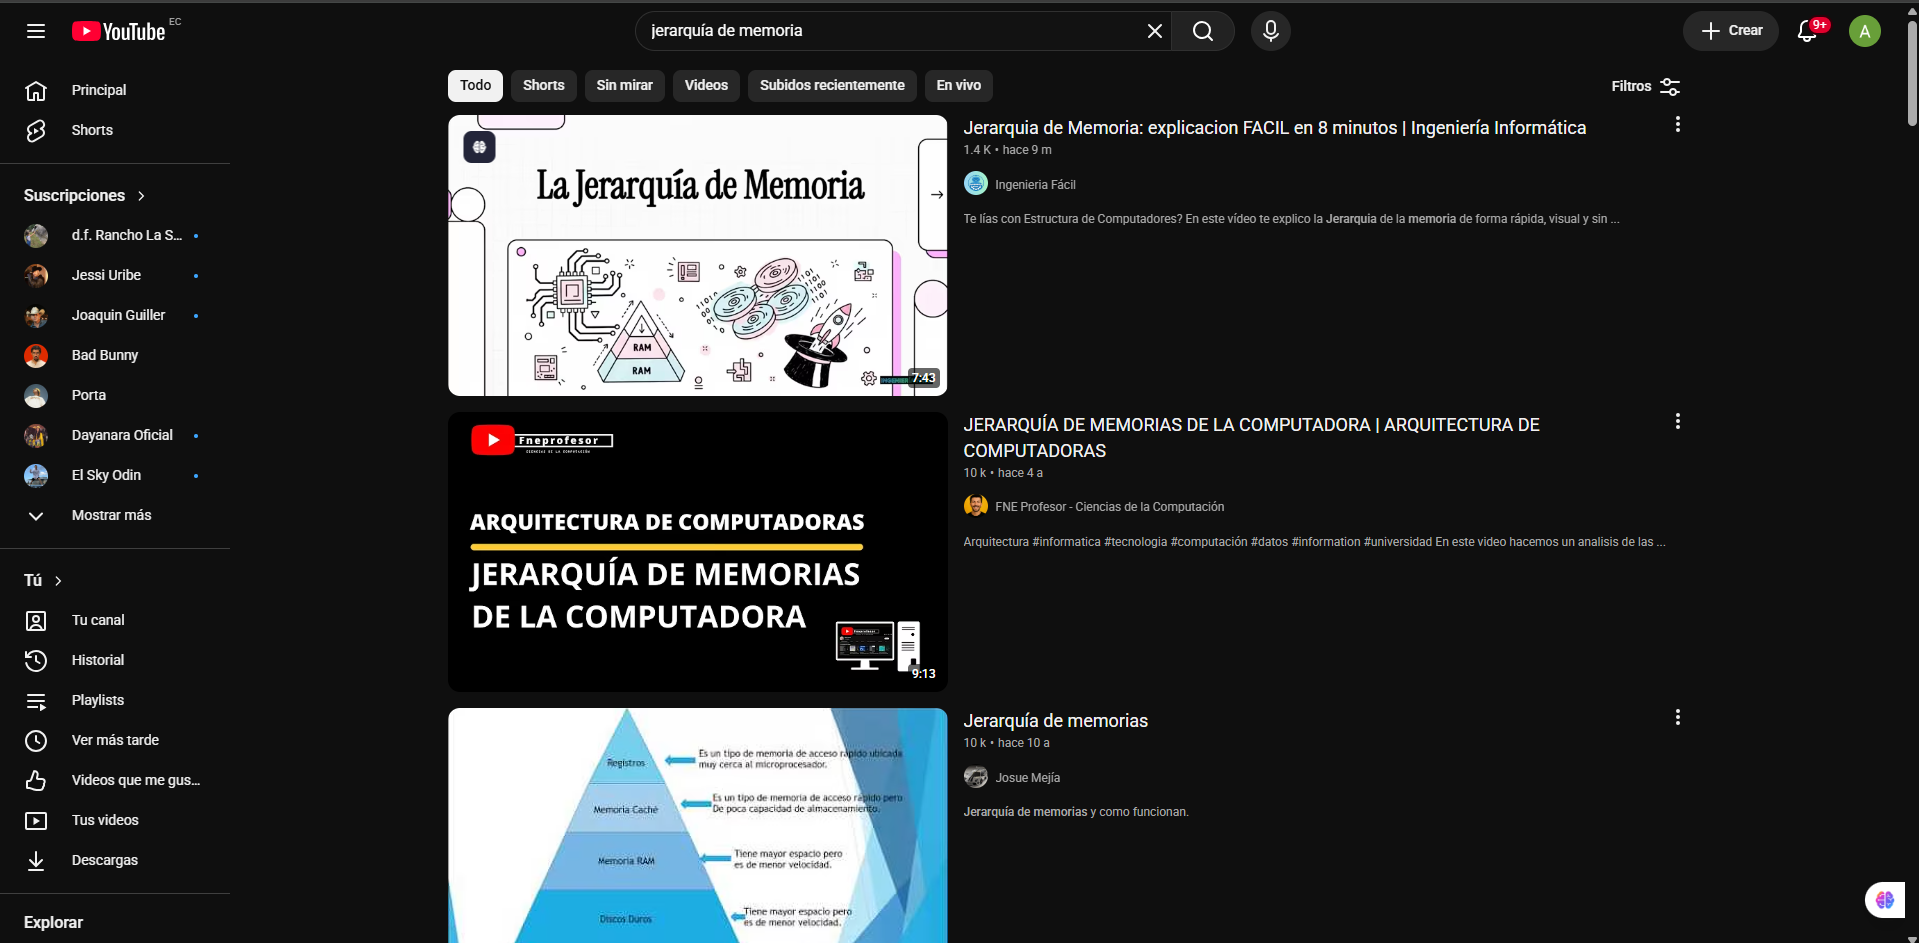
\includegraphics[width=.64\linewidth]{figuras/busqueda.png}

\small Captura 1. Resultados de la búsqueda «jerarquía de memoria».

\begin{minipage}[t]{.47\linewidth}
\centering
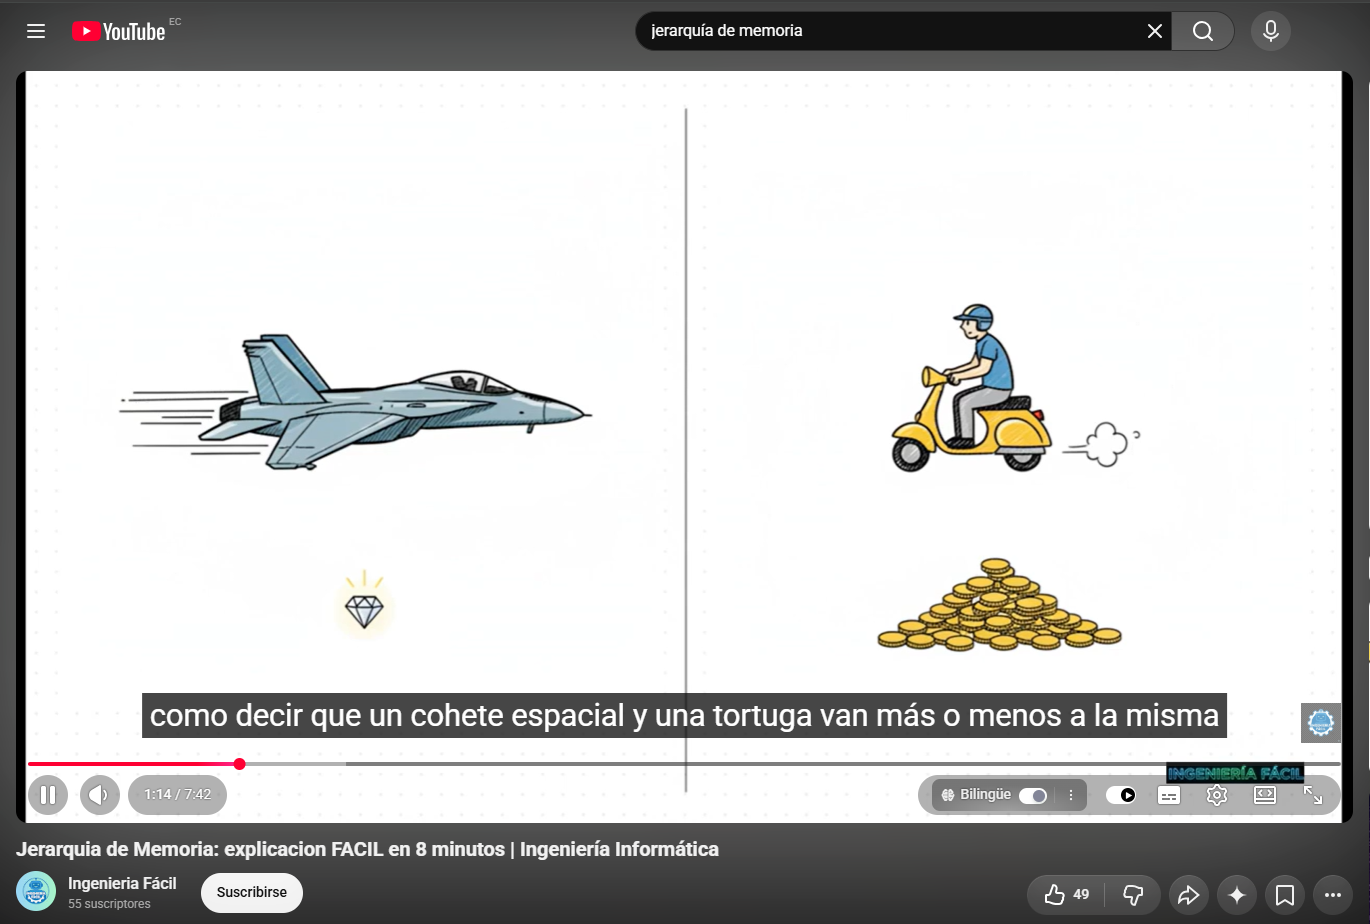
\includegraphics[width=\linewidth]{figuras/reproduccion.png}

Captura 2. Reproducción con controles y subtítulos.
\end{minipage}\hfill
\begin{minipage}[t]{.47\linewidth}
\centering
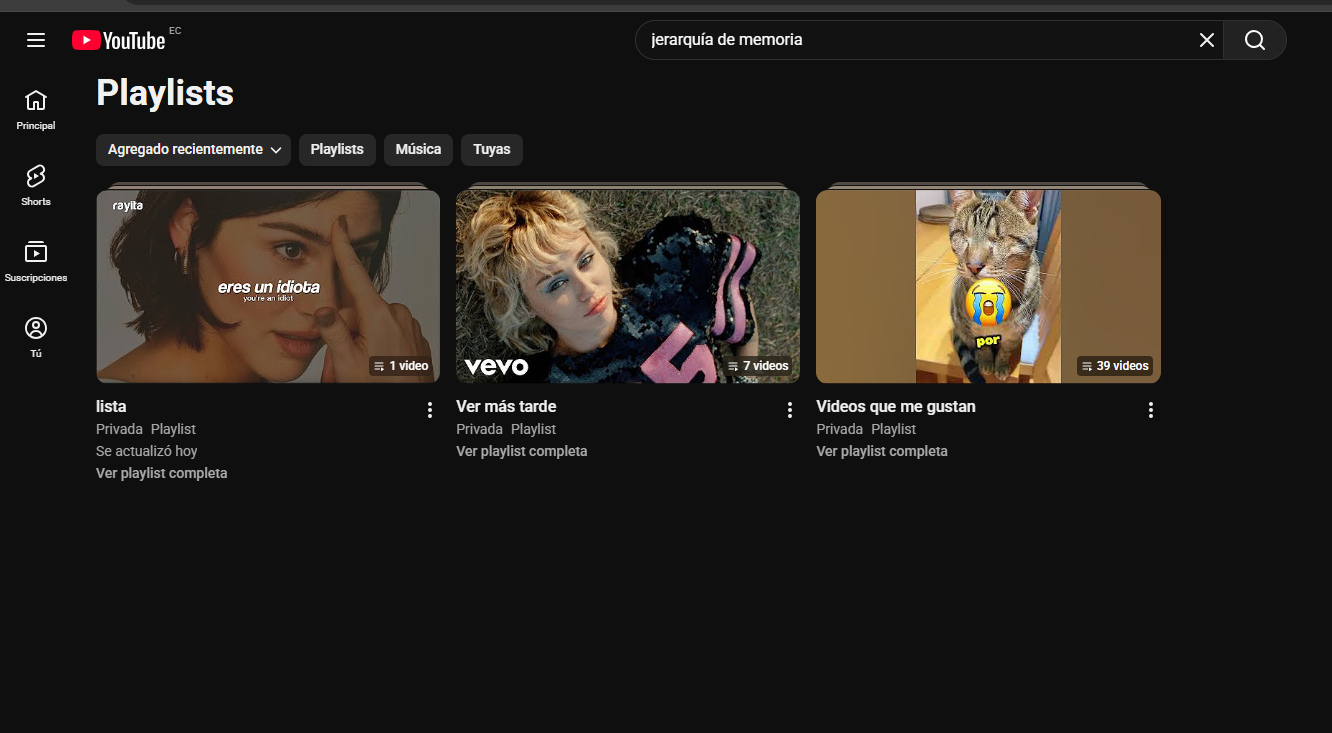
\includegraphics[width=\linewidth]{figuras/listas.png}

Captura 3. Listas de reproducción y conteos.
\end{minipage}
\end{center}
\newpage
\printbibliography[title={Referencias}]

\section*{Declaración de uso de inteligencia artificial}
Se utilizó ChatGPT para aclarar conceptos de ingeniería de requisitos,
preparar borradores del informe y revisar la redacción, los criterios de
aceptación y la coherencia entre secciones. Las capturas corresponden al
uso de YouTube Web. Las métricas son propuestas para el ejercicio y el
informe describe cómo se podrían verificar.
\end{document}
